\documentclass[a4paper,12pt]{article}
\usepackage[utf8]{inputenc}
\usepackage{geometry}
\geometry{
 a4paper,
 left=1.25in,
 right=1.25in,
 top=1in,
 }
\usepackage[croatian,english]{babel}    %za hrvatske naslove
\usepackage[nottoc]{tocbibind}  %za pravilan table of content
\usepackage{graphicx}   %za dodavanje slika
\usepackage{amsmath}    %za matematičke forumele
\usepackage{subcaption} %za dvije slike u jednoj
\usepackage{booktabs}   %za bolje tablice
\usepackage{cite}

\begin{document}

\begin{center}
SVEUČILIŠTE JURJA DOBRILE U PULI 

FAKULTET INFORMATIKE

\vspace{45mm} 

\textbf{Ime Prezime}

\vspace{20mm} 

\textbf{Naslov rad}

\vspace{5mm}
DIPLOMSKI/ZAVRSNI RAD

\vfill

%Upisat tocan mjesec i godinu
Pula, rujan, 2025. godine
\end{center}

\pagenumbering{gobble}
\clearpage
\newpage

\begin{center}
SVEUČILIŠTE JURJA DOBRILE U PULI 

FAKULTET INFORMATIKE

\vspace{45mm} 

\textbf{Neven Nižić}

\vspace{20mm} 

\textbf{"Optimizacija raspodjele projektnih aktivnosti primjenom genetskih algoritama i Monte Carlo simulacije"}

\vspace{5mm}
DIPLOMSKI RAD

\end{center}

\vspace{45mm}

\textbf{JMBAG: 0303118917, izvanredni student}

\textbf{Studijski smjer: Informatika}
\bigskip

\textbf{Kolegij: Modeliranje i simulacije}

\textbf{Znanstveno područje : Društvene znanosti}

\textbf{Znanstveno polje : Informacijske i komunikacijske znanosti}

\textbf{Znanstvena grana : Informacijski sustavi i informatologija}
\bigskip

\textbf{Mentor: dr.sc. Darko Etinger}

\vfill

\begin{center}

%Upisat tocan mjesec i godinu
Pula, rujan, 2025. godine

\end{center}

\pagenumbering{gobble}
\clearpage
\newpage

%Resetirat margine
\restoregeometry

\selectlanguage{croatian}
\begin{abstract}
Upravljanje projektima često uključuje složene odluke vezane uz raspodjelu aktivnosti i resursa, osobito u uvjetima nesigurnosti i vremenskih ograničenja. Tradicionalne metode kao što su PERT i CPM često ne uspijevaju obuhvatiti stohastičku prirodu stvarnih projekata. U ovom radu razvijen je i evaluiran hibridni optimizacijski pristup temeljen na genetskim algoritmima (GA) i Monte Carlo (MC) simulaciji. Kroz dvo-fazni eksperimentalni dizajn, provedena je sustavna usporedba tri modela: nasumične pretrage, jedno-kriterijskog GA usmjerenog isključivo na povrat na investiciju (ROI), te više-kriterijskog GA+MC modela (NSGA-II) koji istovremeno optimizira ROI i rizik trajanja projekta. Rezultati dobiveni na sintetičkim podacima različite složenosti i restriktivnosti pokazuju da, iako jedno-kriterijski GA najučinkovitije maksimizira profit, hibridni GA+MC model uspješno generira Paretov front rješenja koja nude optimalan kompromis između profitabilnosti i trajanja. Nadalje, istraživanje je otkrilo ključan nalaz: pod ekstremno restriktivnim budžetom, robusnost jednostavnijeg, jedno-kriterijskog GA nadmašuje onu složenijeg, više-kriterijskog modela. Rad zaključuje da ne postoji univerzalno superioran model, već da optimalan izbor ovisi o strateškim prioritetima – maksimizaciji profita naspram uravnoteženog upravljanja rizikom.
\end{abstract}
\begin{small}
\textbf{Ključne riječi:} projektno upravljanje, genetski algoritam, Monte Carlo simulacija, više-kriterijska optimizacija, upravljanje rizikom, Paretov front, NSGA-II
\end{small}

\bigskip

\selectlanguage{english}
\begin{abstract}
Project management often involves complex decisions regarding the allocation of activities and resources, especially under conditions of uncertainty and constraints. Traditional methods such as PERT and CPM frequently fail to capture the stochastic nature of real-world projects. This thesis develops and evaluates a hybrid optimization approach based on genetic algorithms (GA) and Monte Carlo (MC) simulation. Through a two-phase experimental design, a systematic comparison of three models was conducted: random search, a single-objective GA focused solely on return on investment (ROI), and a multi-objective GA+MC model (NSGA-II) that simultaneously optimizes ROI and project duration risk. The results, obtained from synthetic data of varying complexity and restrictiveness, show that while the single-objective GA is most effective at maximizing profit, the hybrid GA+MC model successfully generates a Pareto front of solutions offering an optimal trade-off between profitability and duration. Furthermore, the research revealed a key finding: under extremely restrictive budget constraints, the robustness of the simpler, single-objective GA surpasses that of the more complex, multi-objective model. The thesis concludes that there is no universally superior model; rather, the optimal choice depends on strategic priorities—maximizing profit versus balanced risk management.
\end{abstract}
\begin{small}
\textbf{Keywords:} project management, genetic algorithm, Monte Carlo simulation, multi-objective optimization, risk management, Pareto front, NSGA-II
\end{small}

\pagenumbering{gobble}
\clearpage
\newpage

\selectlanguage{croatian}
\tableofcontents
\pagenumbering{gobble}
\clearpage
\newpage

\pagenumbering{arabic}

\section{Uvod}

Upravljanje projektima obuhvaća niz izazova, osobito kada je riječ o optimizaciji raspodjele ograničenih resursa među konkurentskim aktivnostima. Projektni menadžeri često se suočavaju s neizvjesnostima vezanima uz trajanje zadataka, dostupnost resursa i dinamičnost okruženja. Upravo te nesigurnosti zahtijevaju robusne metode koje mogu osigurati učinkovitu alokaciju resursa unatoč stohastičkoj prirodi ulaznih podataka.

\subsection{Motivacija}

Jedan od ključnih problema u upravljanju projektima je kako rasporediti ograničene resurse (vremenske, ljudske, financijske) na skup aktivnosti tako da se minimizira ukupno trajanje projekta ili maksimizira ukupna vrijednost. Klasične determinističke metode često zanemaruju nesigurnosti koje su prisutne u stvarnim projektima, što dovodi do planova koji su nerealni i teško provedivi \cite{Kerzner2017, PMI2021}. Stoga raste interes za primjenom heurističkih i stohastičkih metoda u projektnoj optimizaciji.

\subsection{Rizici i nesigurnosti u projektnom upravljanju}

Neizvjesnost u trajanju aktivnosti, nepredviđeni događaji, promjene prioriteta i ograničeni resursi stvaraju kompleksno i promjenjivo okruženje. Klasifikacija rizika i kvantifikacija njihove vjerojatnosti ključni su za izradu kvalitetnog plana. Zbog toga se uvode stohastičke metode kao što su Monte Carlo simulacija, koje omogućuju analizu različitih scenarija i procjenu vjerojatnosti uspjeha projekta \cite{Vose2008}. Upravo zbog tih izazova, mnogi autori predlažu uporabu kvantitativnih metoda kao što su Monte Carlo simulacije za procjenu vjerojatnih vremenskih i troškovnih odstupanja \cite{Avlijas2008}.

\subsection{Heuristički pristup optimizaciji upravljanja projektima korištenjem kombiniranog stohastičkog modela}

U ovom radu predlaže se heuristički pristup optimizaciji upravljanja projektima korištenjem kombiniranog stohastičkog modela. Pritom se kombiniraju dva komplementarna pristupa:

\begin{itemize}
    \item \textbf{Genetski algoritam (GA)} – koristi se za pronalaženje optimalne ili blizu optimalne raspodjele projektnih aktivnosti, uzimajući u obzir njihovu važnost i vremenska ograničenja. GA su pokazali visoku učinkovitost kod NP-teških problema poput problema ruksaka \cite{Goldberg1989, Mitchell1998}.
    \item \textbf{Monte Carlo simulacija (MCS)} – koristi se za modeliranje neizvjesnosti u trajanju aktivnosti, često koristeći trokutastu distribuciju, posebno kada nije dostupna pouzdana povijesna statistika \cite{Law2015}.
\end{itemize}

Ova kombinacija omogućuje istraživanje velikog prostora rješenja, pri čemu se u svakoj iteraciji genetskog algoritma evaluira kvaliteta rješenja putem više Monte Carlo simulacija. Time se dobiva robusnije rješenje koje bolje odražava nesigurnost u ulaznim podacima.

\subsection{Cilj rada}

Cilj ovog rada je razviti model koji integrira genetski algoritam i Monte Carlo simulaciju u svrhu optimizacije raspodjele projektnih aktivnosti pod uvjetima nesigurnosti. Model se temelji na knapsack formulaciji problema, gdje se svaka aktivnost karakterizira očekivanim trajanjem, varijabilnošću i vrijednošću. Kroz eksperimente će se testirati učinkovitost predloženog pristupa te usporediti dobivena rješenja u kontekstu robustnosti i izvedivosti plana projekta.


Upravljanje projektima je ključna aktivnost u brojnim industrijama, od građevine i IT-a do farmaceutike i financija. Jedan od najzahtjevnijih aspekata upravljanja projektima jest učinkovita raspodjela aktivnosti i resursa kroz vrijeme, pri čemu se mora zadovoljiti niz ograničenja, uključujući budžet, vremenski rok, kapacitete resursa i međusobne ovisnosti između zadataka. U složenim projektima s velikim brojem aktivnosti, tradicionalni pristupi često nisu dostatni jer ne uspijevaju adresirati neizvjesnosti i varijabilnost koje prate realne projekte.

\subsection{Motivacija}

Raspodjela projektnih aktivnosti i resursa u uvjetima nesigurnosti i ograničenja predstavlja NP-težak problem, što znači da se broj mogućih kombinacija rješenja eksponencijalno povećava s veličinom problema. Tradicionalne metode kao što su CPM (Critical Path Method) i PERT (Program Evaluation and Review Technique) podrazumijevaju determinističke vremenske procjene i ne uključuju varijabilnost stvarnih uvjeta, što može dovesti do suboptimalnih ili čak neizvedivih planova.

Potreba za metodama koje mogu obuhvatiti stohastičku prirodu trajanja aktivnosti, dinamiku projektnog okruženja i složene međusobne odnose među aktivnostima, motivira primjenu naprednih optimizacijskih i simulacijskih tehnika.

\subsection{Rizici i nesigurnosti u projektnom upravljanju}

U stvarnim projektima, trajanja aktivnosti često nisu poznata unaprijed s potpunom sigurnošću. Kašnjenja, nedostatak resursa, promjene u specifikacijama ili nepredviđene okolnosti mogu značajno utjecati na tijek projekta. Zbog toga je važno uključiti kvantitativne metode za procjenu rizika i analizu nesigurnosti. Upravo tu se Monte Carlo simulacija ističe kao snažan alat koji omogućuje evaluaciju raspodjele mogućih ishoda i procjenu vjerojatnosti završetka projekta unutar zadanih rokova.

\subsection{Monte Carlo simulacija i genetski algoritmi}

Monte Carlo simulacija koristi slučajne uzorke za kvantificiranje nesigurnosti u modelima i omogućuje realističnije procjene vremenskih i troškovnih distribucija. U kontekstu projektnog upravljanja, ova metoda može simulirati tisuće mogućih scenarija izvedbe aktivnosti na temelju probabilističkih ulaza (npr. optimističnog, realnog i pesimističnog trajanja).

Genetski algoritmi (GA) predstavljaju jednu od najčešće korištenih metaheurističkih metoda za rješavanje složenih problema optimizacije. Temelje se na principima evolucije i prirodne selekcije te su učinkoviti u pretraživanju velikih prostora rješenja, što ih čini pogodnima za optimizaciju projektnih rasporeda.

\subsection{Cilj rada}

Cilj ovog rada je razviti model koji kombinira genetski algoritam s Monte Carlo simulacijom radi dobivanja robusnog plana raspodjele aktivnosti u projektu. Kombinacija ovih dviju metoda omogućava simultano:
\begin{itemize}
    \item optimiziranje projektnih rasporeda u uvjetima složenih ograničenja,
    \item kvantifikaciju rizika i nesigurnosti u izvedbi projekta,
    \item donošenje boljih odluka u upravljanju resursima.
\end{itemize}

Predloženi pristup testira se na simuliranim podacima i evaluira s obzirom na pouzdanost završetka projekta unutar vremenskog roka i efikasnost raspodjele resursa.


\newpage

\section{Poglavlje}

Ovako citiram Pytorch \cite{pytorch} i Numpy \cite{numpy}. Ovako citiram vise stvari \cite{backpropagation_1986,neuronska_mreza_1943, perceptron_1958}. Lorem ipsum dolor sit amet, consectetur adipiscing elit, sed do eiusmod tempor incididunt ut labore et dolore magna aliqua. Ut enim ad minim veniam, quis nostrud exercitation ullamco laboris nisi ut aliquip ex ea commodo consequat.

%ht! -> ako zelim da mi slika bude vise manje na istom mjestu gdje sam je stavio u source code-u
%width=\textwidth -> sirina slike jednaka stranici, ovisno o slici moze se koristit i scale=0.6 itd.
\begin{figure}[ht!]
    \centering
    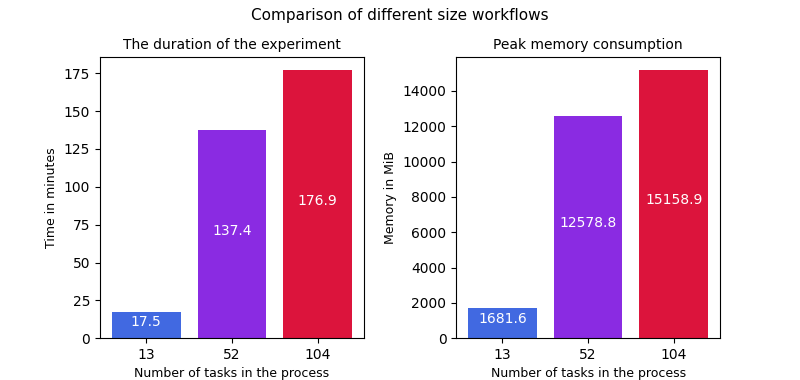
\includegraphics[width=\textwidth]{slike/test-slika.png}
    \caption{Ovo je naslov slike}
    \label{fig:slika}
\end{figure}

Ovako referenciram sliku \ref{fig:slika}. Ut enim ad minim veniam, quis nostrud exercitation ullamco laboris nisi ut aliquip ex ea commodo consequat. Duis aute irure dolor in reprehenderit in voluptate velit esse cillum dolore eu fugiat nulla pariatur.

\subsection{Podpoglavlje}

Lorem ipsum dolor sit amet, consectetur adipiscing elit, sed do eiusmod tempor incididunt ut labore et dolore magna aliqua. Ut enim ad minim veniam, quis nostrud exercitation ullamco laboris nisi ut aliquip ex ea commodo consequat. Duis aute irure dolor in reprehenderit in voluptate velit esse cillum dolore eu fugiat nulla pariatur.

%Tablice su malo problematicne u latex-u, preporucam https://www.tablesgenerator.com/

\begin{table}[ht!]
\centering
\begin{tabular}{@{}cccc@{}}
\toprule
 Test      & Varijabla 2 & Varijabla 3 & Varijabla 4 \\ \midrule
Test 1 & 2.12341     & 3.12341234  & 4.1235      \\
Test 2 & 5.123       & 6.34        & 7.123       \\ \bottomrule
\end{tabular}
\caption{Ovo je naslov tablice}
\label{tab:my-table}
\end{table}

Ovako referenciram tablicu \ref{tab:my-table}. Ut enim ad minim veniam, quis nostrud exercitation ullamco laboris nisi ut aliquip ex ea commodo consequat. Duis aute irure dolor in reprehenderit in voluptate velit esse cillum dolore eu fugiat nulla pariatur.

\subsubsection{PodPodPoglavlje}\label{pod-pod-poglavlje}

Lorem ipsum dolor sit amet, consectetur adipiscing elit, sed do eiusmod tempor incididunt ut labore et dolore magna aliqua. Ut enim ad minim veniam, quis nostrud exercitation ullamco laboris nisi ut aliquip ex ea commodo consequat. Duis aute irure dolor in reprehenderit in voluptate velit esse cillum dolore eu fugiat nulla pariatur. Excepteur sint occaecat cupidatat non proident, sunt in culpa qui officia deserunt mollit anim id est laborum. Lorem ipsum dolor sit amet, consectetur adipiscing elit, sed do eiusmod tempor incididunt ut labore et dolore magna aliqua. Ut enim ad minim veniam, quis nostrud exercitation ullamco laboris nisi ut aliquip ex ea commodo consequat. Duis aute irure dolor in reprehenderit in voluptate velit esse cillum dolore eu fugiat nulla pariatur. 

\subsection{Drugo podpoglavlje}

Ovako mogu referencirat poglavlje \ref{pod-pod-poglavlje} u radu. I ako mi treba fusnota\footnote{Ovo je fusnota...}. Excepteur sint occaecat cupidatat non proident, sunt in culpa qui officia deserunt mollit anim id est laborum. Lorem ipsum dolor sit amet, consectetur adipiscing elit, sed do eiusmod tempor incididunt ut labore et dolore magna aliqua. Ut enim ad minim veniam, quis nostrud exercitation ullamco laboris nisi ut aliquip ex ea commodo consequat. Duis aute irure dolor in reprehenderit in voluptate velit esse cillum dolore eu fugiat nulla pariatur. Excepteur sint occaecat cupidatat non proident, sunt in culpa qui officia deserunt mollit anim id est laborum. Lorem ipsum dolor sit amet, consectetur adipiscing elit, sed do eiusmod tempor incididunt ut labore et dolore magna aliqua. Ut enim ad minim veniam, quis nostrud exercitation ullamco laboris nisi ut aliquip ex ea commodo consequat. Duis aute irure dolor in reprehenderit in voluptate velit esse cillum dolore eu fugiat nulla pariatur. Excepteur sint occaecat cupidatat non proident, sunt in culpa qui officia deserunt mollit anim id est laborum. Lorem ipsum dolor sit amet, consectetur adipiscing elit, sed do eiusmod tempor incididunt ut labore et dolore magna aliqua. Ut enim ad minim veniam, quis nostrud exercitation ullamco laboris nisi ut aliquip ex ea commodo consequat. Duis aute irure dolor in reprehenderit in voluptate velit esse cillum dolore eu fugiat nulla pariatur.

\newpage

\section{Novo poglavlje}
%Prvi paragraf
Lorem ipsum dolor sit amet, consectetur adipiscing elit, sed do eiusmod tempor incididunt ut labore et dolore magna aliqua. Ut enim ad minim veniam, quis nostrud exercitation ullamco laboris nisi ut aliquip ex ea commodo consequat. Duis aute irure dolor in reprehenderit in voluptate velit esse cillum dolore eu fugiat nulla pariatur. Excepteur sint occaecat cupidatat non proident, sunt in culpa qui officia deserunt mollit anim id est laborum. Lorem ipsum dolor sit amet, consectetur adipiscing elit, sed do eiusmod tempor incididunt ut labore et dolore magna aliqua. Ut enim ad minim veniam, quis nostrud exercitation ullamco laboris nisi ut aliquip ex ea commodo consequat. Duis aute irure dolor in reprehenderit in voluptate velit esse cillum dolore eu fugiat nulla pariatur. Excepteur sint occaecat cupidatat non proident, sunt in culpa qui officia deserunt mollit anim id est laborum. Lorem ipsum dolor sit amet, consectetur adipiscing elit, sed do eiusmod tempor incididunt ut labore et dolore magna aliqua. Ut enim ad minim veniam, quis nostrud exercitation ullamco laboris nisi ut aliquip ex ea commodo consequat. Duis aute irure dolor in reprehenderit in voluptate velit esse cillum dolore eu fugiat nulla pariatur. Excepteur sint occaecat cupidatat non proident, sunt in culpa qui officia deserunt mollit anim id est laborum.

%Drugi paragraf
Lorem ipsum dolor sit amet, consectetur adipiscing elit, sed do eiusmod tempor incididunt ut labore et dolore magna aliqua. Ut enim ad minim veniam, quis nostrud exercitation ullamco laboris nisi ut aliquip ex ea commodo consequat. Duis aute irure dolor in reprehenderit in voluptate velit esse cillum dolore eu fugiat nulla pariatur. Excepteur sint occaecat cupidatat non proident, sunt in culpa qui officia deserunt mollit anim id est laborum. Lorem ipsum dolor sit amet, consectetur adipiscing elit, sed do eiusmod tempor incididunt ut labore et dolore magna aliqua. Ut enim ad minim veniam, quis nostrud exercitation ullamco laboris nisi ut aliquip ex ea commodo consequat. Duis aute irure dolor in reprehenderit in voluptate velit esse cillum dolore eu fugiat nulla pariatur. Excepteur sint occaecat cupidatat non proident, sunt in culpa qui officia deserunt mollit anim id est laborum. Lorem ipsum dolor sit amet, consectetur adipiscing elit, sed do eiusmod tempor incididunt ut labore et dolore magna aliqua. Ut enim ad minim veniam, quis nostrud exercitation ullamco laboris nisi ut aliquip ex ea commodo consequat. Duis aute irure dolor in reprehenderit in voluptate velit esse cillum dolore eu fugiat nulla pariatur. Excepteur sint occaecat cupidatat non proident, sunt in culpa qui officia deserunt mollit anim id est laborum. Lorem ipsum dolor sit amet, consectetur adipiscing elit, sed do eiusmod tempor incididunt ut labore et dolore magna aliqua. Ut enim ad minim veniam, quis nostrud exercitation ullamco laboris nisi ut aliquip ex ea commodo consequat. Duis aute irure dolor in reprehenderit in voluptate velit esse cillum dolore eu fugiat nulla pariatur. Ut enim ad minim veniam, quis nostrud exercitation ullamco laboris nisi ut aliquip ex ea commodo consequat. Duis aute irure dolor in reprehenderit in voluptate velit esse cillum dolore eu fugiat nulla pariatur. Ut enim ad minim veniam, quis nostrud exercitation ullamco laboris nisi ut aliquip ex ea commodo consequat. Duis aute irure dolor in reprehenderit in voluptate velit esse cillum dolore eu fugiat nulla pariatur.
\newpage

\section{Zaključak}

U ovom diplomskom radu predstavili smo kompleksan pristup optimizaciji raspodjele projektnih aktivnosti koristeći kombinaciju genetskih algoritama i Monte Carlo simulacije. Cilj je bio razviti model koji uzima u obzir nesigurnost u trajanju, troškovima i vrijednosti zadataka, te u okviru zadanih ograničenja vremena, budžeta i raspoloživih resursa maksimizira ukupnu vrijednost projekta.

Kroz detaljnu analizu problematike i pregled postojeće literature, identificirali smo ključne izazove u upravljanju projektima, posebice u segmentu neizvjesnosti i složenosti optimizacije. Implementacijom metaheurističkih metoda, u ovom slučaju genetskih algoritama \cite{Goldberg1989, Mitchell1998}, omogućili smo efikasno pretraživanje velikog prostora rješenja, dok je Monte Carlo simulacija služila za kvantitativno modeliranje rizika i nesigurnosti \cite{Miller2009, Avlijas2008}, dajući time realističniju procjenu performansi optimizacijskog rješenja.

Praktična implementacija rezultirala je modelom koji omogućuje donošenje informiranih odluka u planiranju i upravljanju projektima, pružajući projektnim menadžerima alate za bolje usklađivanje ciljeva i ograničenja. Pokazalo se da je kombinacija ovih metoda učinkovita u pronalasku balansiranih rješenja koja maksimiziraju povrat ulaganja, uz minimizaciju rizika od prekoračenja budžeta ili rokova.

Iako su postignuti rezultati zadovoljavajući, postoje brojna područja za buduća istraživanja i unaprjeđenja, među kojima izdvajamo:
\begin{itemize}
    \item Proširenje modela na dinamičke uvjete projekata koji se mijenjaju tijekom vremena, uključujući nepredvidive vanjske utjecaje.
    \item Integracija dodatnih metaheurističkih i hibridnih algoritama, poput algoritama rojčaste inteligencije ili simuliranog kaljenja, radi poboljšanja kvalitete rješenja \cite{Gandomi2013}.
    \item Primjena tehnika strojnog učenja za preciznije predviđanje distribucija nesigurnosti i automatsku adaptaciju parametara optimizacije.
    \item Razvoj softverskih alata s intuitivnim korisničkim sučeljem za praktičnu primjenu predloženih metoda u realnim projektnim okruženjima.
\end{itemize}

Zaključno, ovaj rad potvrđuje važnost primjene naprednih algoritamskih rješenja u upravljanju projektima, posebno u uvjetima nesigurnosti, te doprinosi boljem razumijevanju i praktičnoj primjeni optimizacijskih i simulacijskih metoda u području projektne ekonomike i menadžmenta. Kao što ističe Kerzner \cite{Kerzner2017}, učinkovito upravljanje projektima u suvremenom okruženju zahtijeva kombinaciju tradicionalnih i naprednih pristupa, a naš model pruža značajan doprinos u tom smjeru.



\newpage

\bibliographystyle{unsrt}
\bibliography{literatura}
\newpage

%Automatski generira listu svih slika
\listoffigures
\newpage

%Automatski generira listu svih tablica
\listoftables
\newpage


\end{document}
